\documentclass{standalone}
\usepackage{graphicx}	
\usepackage{amssymb, amsmath}
\usepackage{color}

\usepackage{tikz}
\usetikzlibrary{intersections, backgrounds}

\definecolor{light}{RGB}{220, 188, 188}
\definecolor{mid}{RGB}{185, 124, 124}
\definecolor{dark}{RGB}{143, 39, 39}
\definecolor{highlight}{RGB}{180, 31, 180}
\definecolor{gray10}{gray}{0.1}
\definecolor{gray20}{gray}{0.2}
\definecolor{gray30}{gray}{0.3}
\definecolor{gray40}{gray}{0.4}
\definecolor{gray60}{gray}{0.6}
\definecolor{gray70}{gray}{0.7}
\definecolor{gray80}{gray}{0.8}
\definecolor{gray90}{gray}{0.9}
\definecolor{gray95}{gray}{0.95}

\newcommand*{\offset}{0.025}

\begin{document}

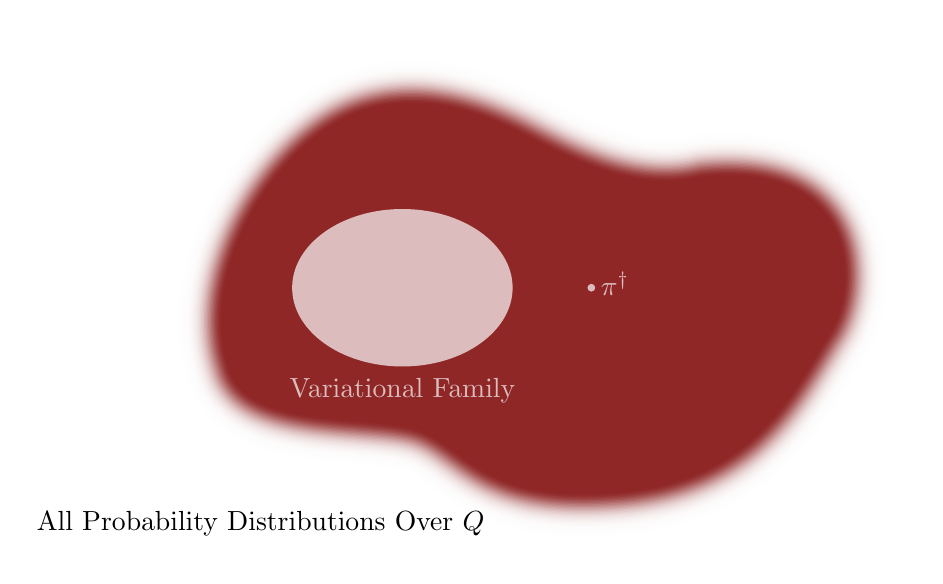
\begin{tikzpicture}[scale=0.2, thick]               
 \pgfmathsetmacro{\dx}{18}
 
 \foreach \i in {1, 0.975, ..., 0} {
   \pgfmathsetmacro{\prop}{100 * exp(-10.0 * \i * \i)};
   \colorlet{custom}{dark!\prop!white};
   \draw[line width={40 * \i}, color=custom] 
     (-20, -2)
    .. controls (-22, 4) and (-17, 12) .. (-12, 14)  
    .. controls (-7, 16) and (-2, 13) .. (0, 12)
    .. controls (2, 11) and (6, 9) .. (10, 10)
    .. controls (20, 11) and (20, 3) .. (18, 0)
    .. controls (15.5, -4) and (13, -9.5) .. (4, -10)
    .. controls (-4, -10.5) and (-5, -7) .. (-8, -6)
    .. controls (-11, -5) and (-19, -6) .. (-20, -2);
  }
  
  \fill [dark] (-20, -2)
    .. controls (-22, 4) and (-17, 12) .. (-12, 14)  
    .. controls (-7, 16) and (-2, 13) .. (0, 12)
    .. controls (2, 11) and (6, 9) .. (10, 10)
    .. controls (20, 11) and (20, 3) .. (18, 0)
    .. controls (15.5, -4) and (13, -9.5) .. (4, -10)
    .. controls (-4, -10.5) and (-5, -7) .. (-8, -6)
    .. controls (-11, -5) and (-19, -6) .. (-20, -2);
    
  \node [] at (-18, -12) { All Probability Distributions Over $Q$ };
    
  \fill[light] (-9, 3) circle (7 and 5);
  \node[light] at (-9, -3.5) {Variational Family};
  
  \fill[light] (3, 3) circle (7pt); 
  \node[light] at (4.5, 3.25) {$\pi^{\dagger}$}; 
  
\end{tikzpicture}

\end{document}   